\section{Clustering using \acs*{optics}}\label{sec:impl-optics}

\begin{figure}[htp] % htp = hier (h), top (t), oder auf einer eigenen Seite (p).
    \centering
    \includesvg[width=0.5\textwidth]{images/OPTICS/OPTICS_procedure.svg}
    \caption{First, the first page of each document is converted to an image.
    Then the image is preprocessed, i.e. conversion to greyscale and resizing.
    }
    \label{fig:OPTICS_procedure}
\end{figure}

Similar to the approach from \cite{OPTICS1999}, \ac{optics} was used to cluster the images of the first page of documents in this work.
The procedure is displayed in \autoref{fig:OPTICS_procedure}.
There were two different preprocessing approaches:
\begin{enumerate}
    \item \label{pt:32}The images were first preprocessed to 32x32 greyscale pixels (cf. \cite{OPTICS1999}) as visualized in \autoref{fig:preprocessed_docs_32x32}
    and afterwards compressed to 13-dimensional vectors using \ac{pca}.
    \item \label{pt:eigendocs}The technique \eigendocs{} from \autoref{subsec:eigenface} 
    was used to compress the images to 13-dimensional greyscale images as displayed in \autoref{fig:preprocessed_docs_eigendocs}.
\end{enumerate}


% preprocessed images
\begin{figure}[htp] % htp = hier (h), top (t), oder auf einer eigenen Seite (p).
    \centering
    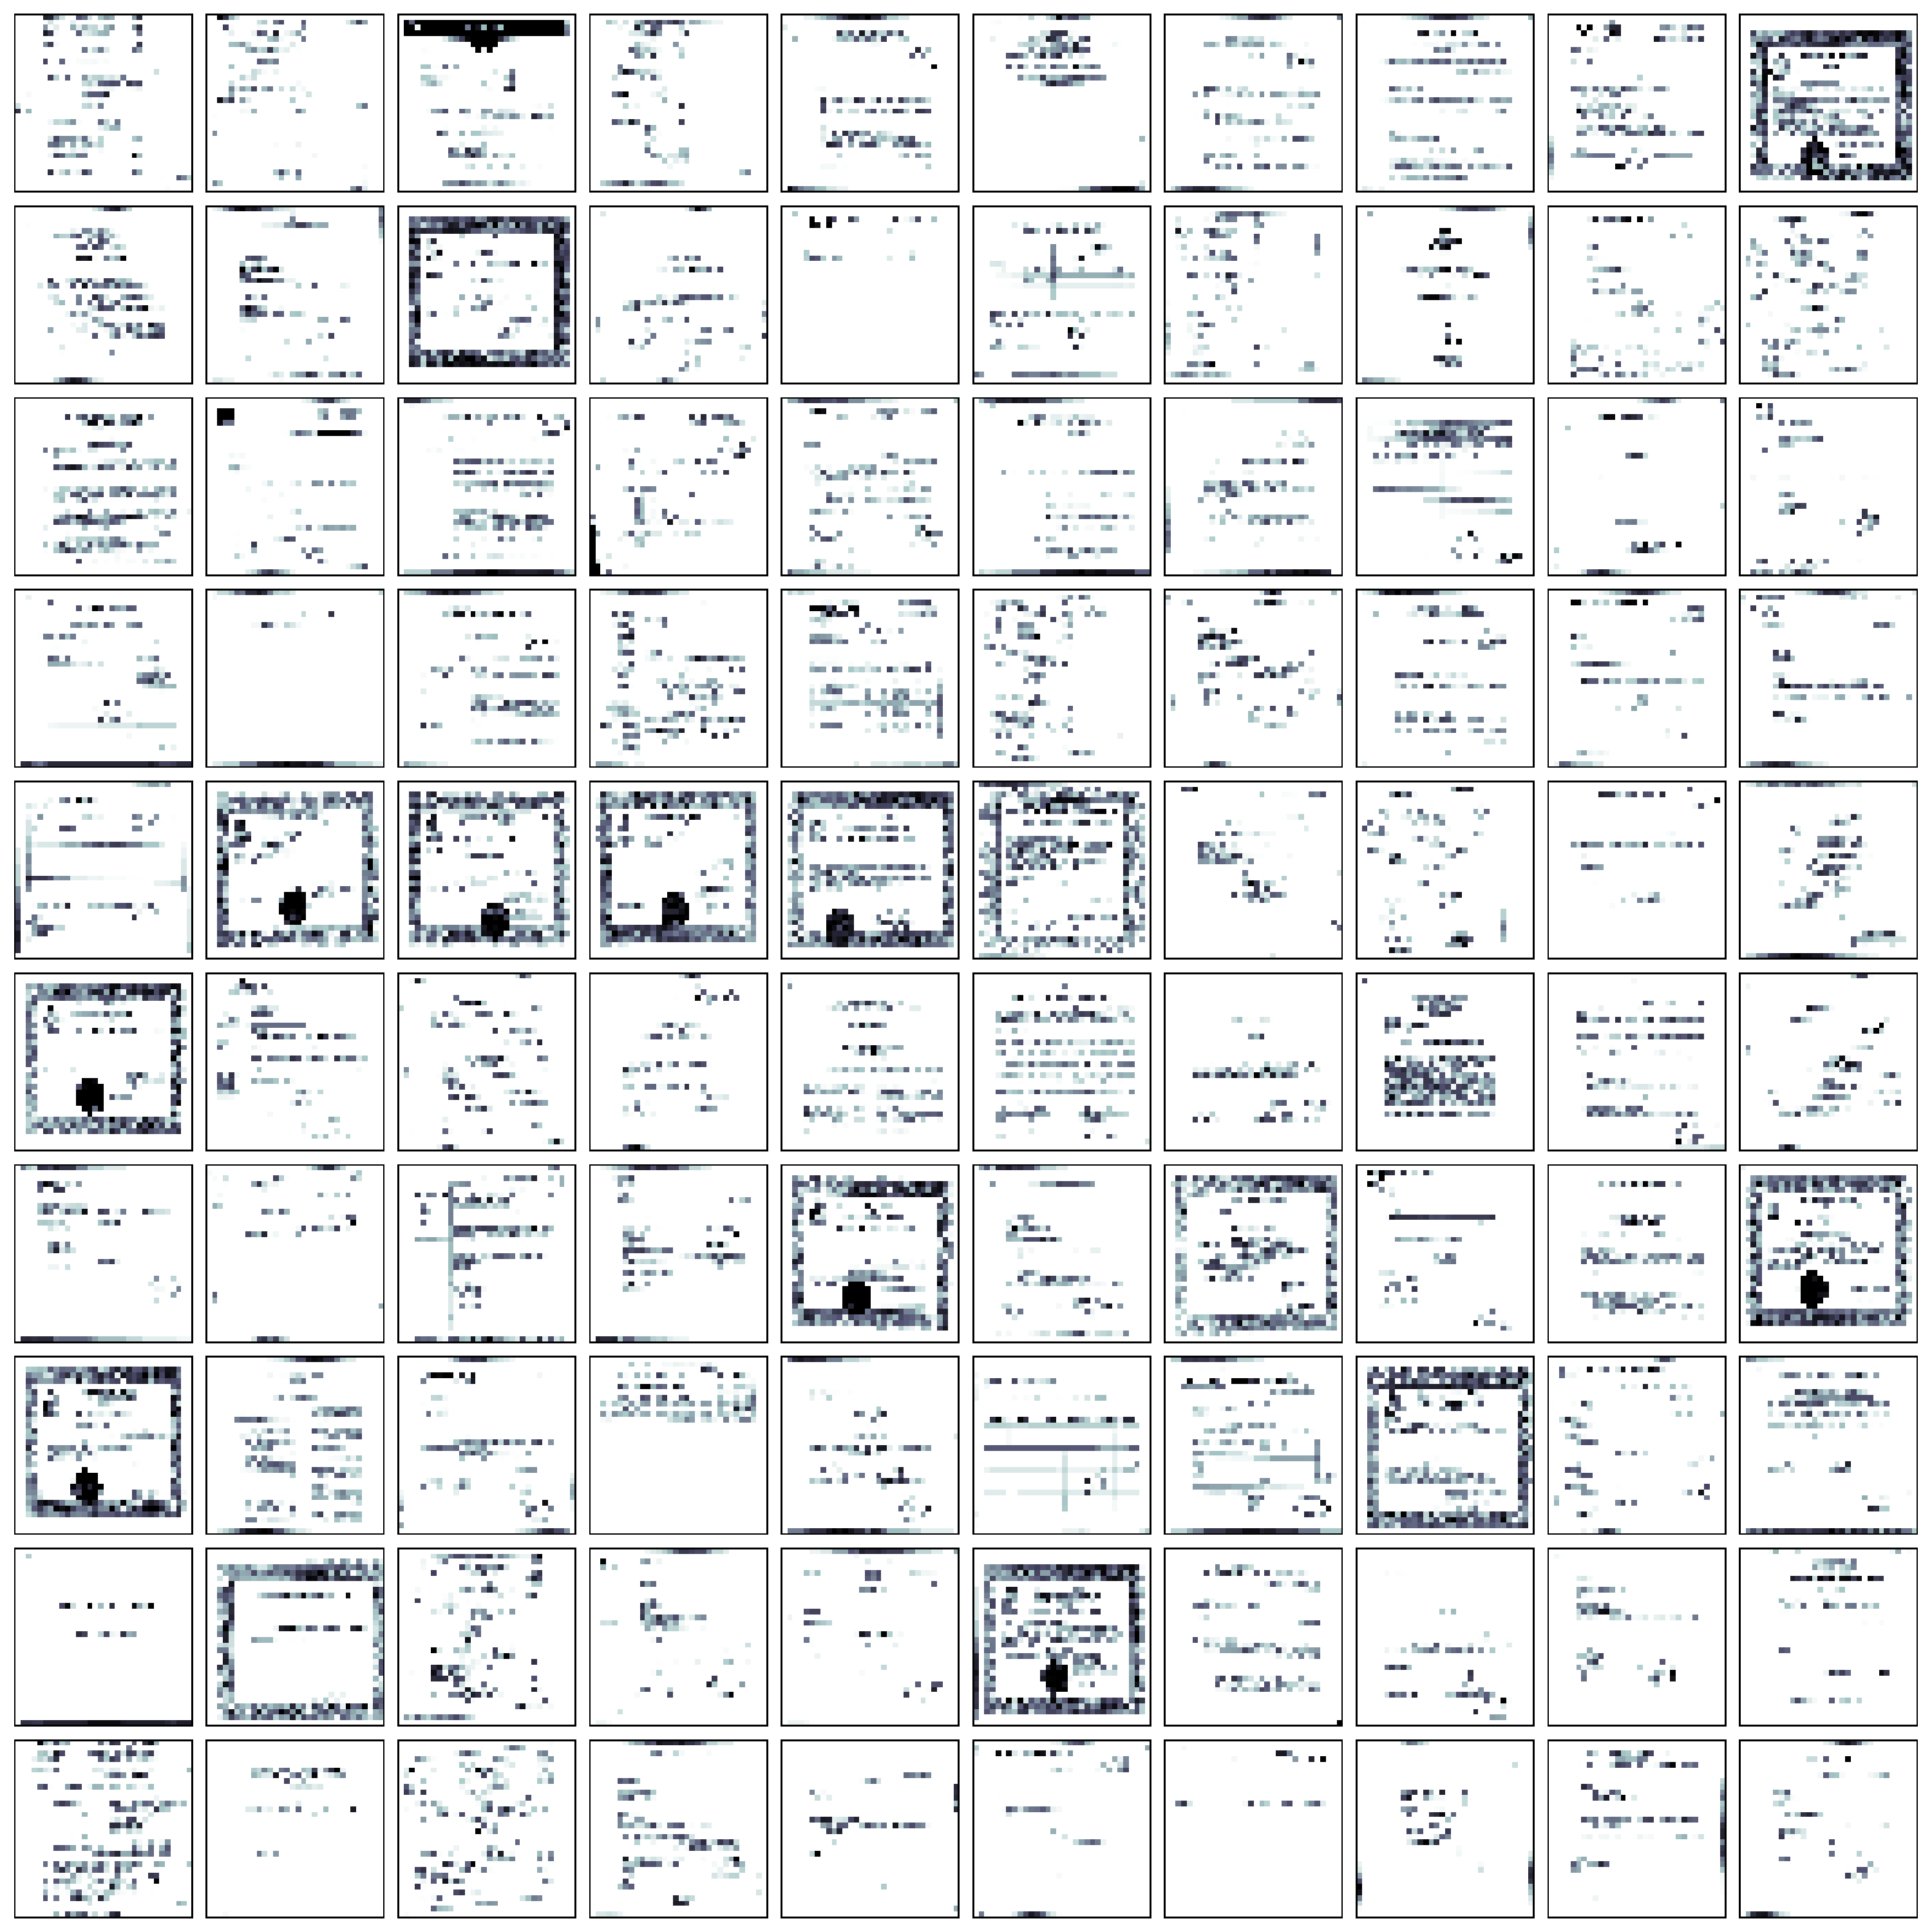
\includegraphics[width=0.4\textwidth]{images/OPTICS/32x32/preprocessed_docs.pdf}
    \caption{The first 100 documents of the dataset compressed to 32x32 greyscale pixels.
    }
    \label{fig:preprocessed_docs_32x32}
\end{figure}

The reachability distance ordered by \ac{optics} is displayed in \autoref{fig:reachability_plots}.
The resulting clusters are displayed in \autoref{fig:optics_cluster}.

% reachability plot
\begin{figure}%
    \centering
    \subfloat[\centering The reachability plot of the documents preprocessed according to \autoref{pt:32}.]{{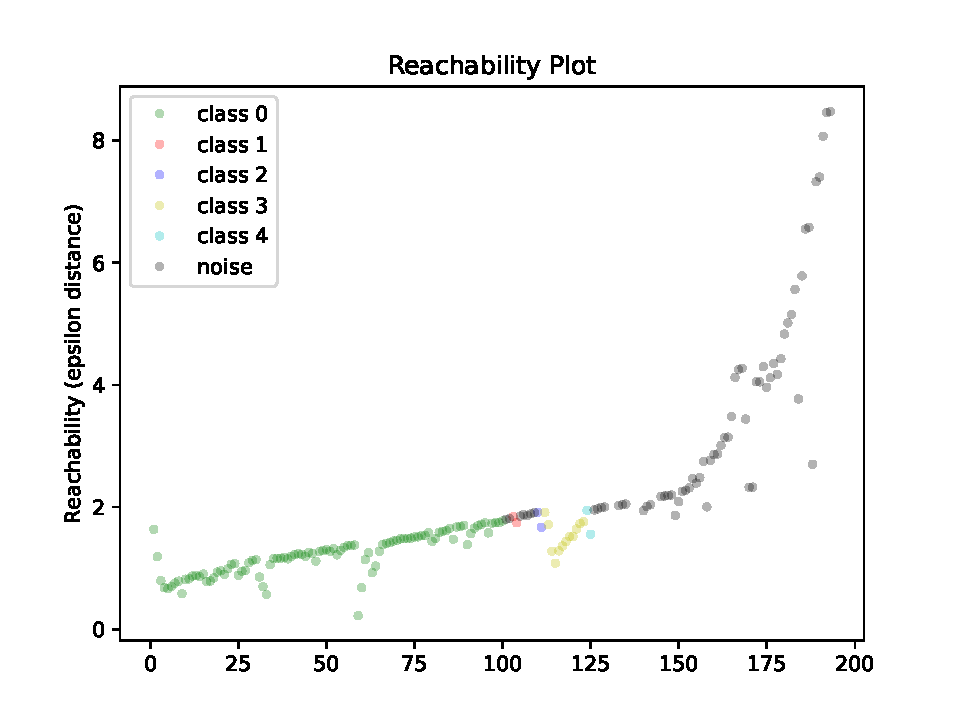
\includegraphics[width=5cm]{images/OPTICS/32x32/reachability_plot_32x32_pca_13dim.pdf} }}%
    \qquad
    \subfloat[\centering The reachability plot of the documents preprocessed according to \autoref{pt:eigendocs}.]{{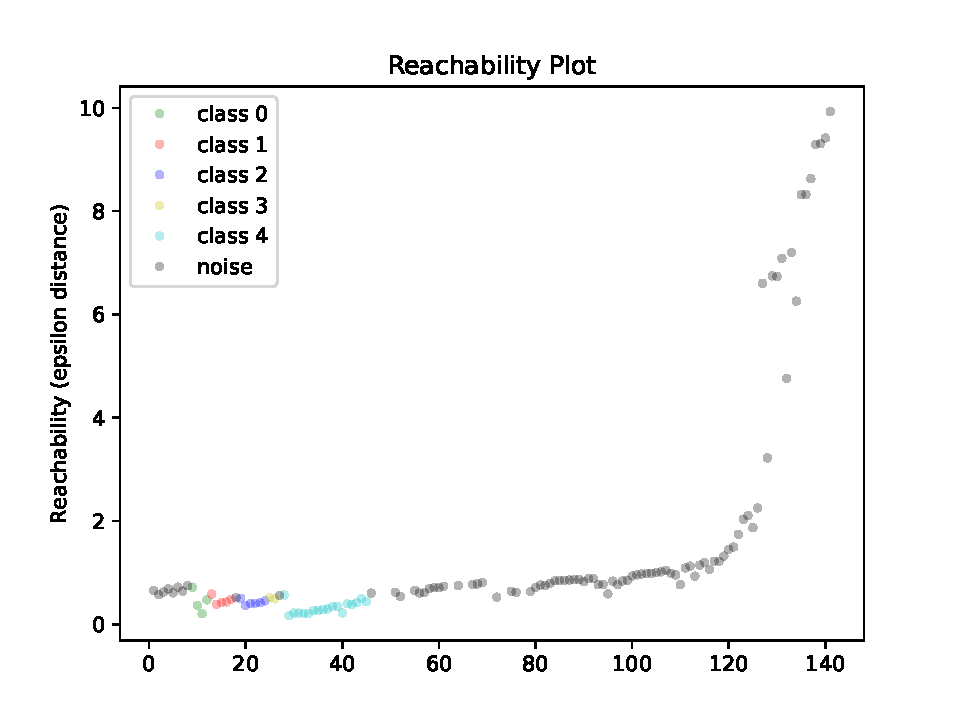
\includegraphics[width=5cm]{images/OPTICS/eigendocs/reachability_plot_13dim_eigendocs.pdf} }}%
    \caption{The plot was created using the \ac{optics} algorithm from the Python library scikit-learn.
    It shows the reachability distance of each document to its predecessor in the order list.}%
    \label{fig:reachability_plots}%
\end{figure}

% code
The configurations used when initializing an \ac{optics} model greatly influence the clusters returned.
The user has to consider the increase of complexity when choosing a high \texttt{max\_eps} value.
The way the reachability plot is used to extract cluster is dependent on the \texttt{cluster\_method}, 
whereas \texttt{min\_smaples} and \texttt{eps} influence the cluster sizes and number of cluster found for a given clustering approach.
The code to initialize an exemplartary \ac{optics} model is displayed in \lst{lst:optics_model}.

\begin{listing}[htp]
    \begin{minted}{python3}
        optics_model = OPTICS(cluster_method='dbscan', min_samples=2, max_eps=10, 
            eps=0.5)
    \end{minted}
    \caption{Initialization of the \ac{optics} model.
    One can choose either \texttt{dbscan} or \texttt{xi} as clustering method.
    The number of minimum samples in a cluster corresponds to \textit{minPts}.
    The parameter \texttt{max\_eps} is infinity as default, but can be specified by the user to reduce complexity and runtime.
    According to literature, \texttt{max\_eps} should be big enough to include almost all points in a cluster.
    The value of \texttt{eps} define the distance between two points to still be considered neighbors 
    and can be chosen consulting the reachability plot.
    }
    \label{lst:optics_model}
\end{listing}
